\section{Решение дифференциальных уравнений}

\begin{ex}
Экспериментально установлено, что при движении пули массы $m$ в деревянной доске сила сопротивления пропорциональна скорости пули по закону $\vec{F} = - \alpha \vec{v}$. Какой путь пройдет пуля в доске до остановки, если начальная скорость пули $v_0$?
\begin{ans}
$x(t) = \frac{mv_0}{\alpha}\left( 1 - e^{-\alpha t /m}\right)$, $s = mv_0/\alpha$
\end{ans}
\end{ex}

\begin{ex}
При движении тел в воздухе на них действует сила сопротивления пропорциональная квадрату скорости $F = - \alpha v^2$. По какому закону изменяются скорость и пройденный путь телом массы $m$ при движении без начальной скорости?
\begin{ans}
$v(t) = \sqrt{\frac{mg}{\alpha}} \tanh (kt/m)$, $s = \frac{m}{\alpha} \sqrt{\frac{mg}{\alpha}} \cosh^2 (kt/m)$
\end{ans}
\end{ex}

%Черепанов
\begin{ex}
Стальной шарик падает с высоты $h$ с нулевой начальной скоростью на стальную плиту. Сопротивление воздуха пропорционально квадрату скорости шарика, коэффициент пропорциональности $k$. Удар о плиту абсолютно упругий. На какую высоту $\Delta h$ шарик не долетит до начального положения при первом отскоке?
\begin{ans}
$\Delta h = \frac{1}{2\beta} \log \frac{e^{2\beta h}}{2 - e^{-2\beta h}}$, $\beta = k/m$
\end{ans}
\end{ex}

%www.math24.ru
\begin{ex}
В начальный момент цепочка длиной $L$ свисает над краем стола таким образом, что сила тяжести уравновешена силой трения. В результате небольшого смещения $\varepsilon$ цепочка начинает скользить. Определить время $T$, за которое цепочка полностью соскользнет со стола. Коэффициент трения между цепочкой и поверхностью стола равен $\mu$.
\begin{ans}
$T = \sqrt{\frac{L}{(1+\mu) g}} \arccosh \frac{L}{\varepsilon (1+\mu)g} = \sqrt{\frac{L}{(1+\mu) g}} \log \left[ \frac{L}{\varepsilon (1+\mu) g} - \sqrt{\frac{L^2}{\varepsilon^2 (1+\mu)^2 g^2} - 1}\right]$
\end{ans}
\end{ex}

\begin{ex}
\hspace{0pt} \\
\begin{minipage}{.65\textwidth}
Бачок имеет форму параллелепипеда с площадью основания $S^*$. При его наполнении водой поднимается поплавок, который постепенно закрывает кран подачи воды. Для простоты будем считать, что с увеличением уровня воды $h$ в бачке площадь отверстия крана уменьшается по линейному закону $S = S_0 (1 - h/h_{\max})$. Скорость подачи воды постоянна и равна $v$. За какое время бачок полностью наполнится водой?
\end{minipage}
\begin{minipage}{.35\textwidth}
\centering
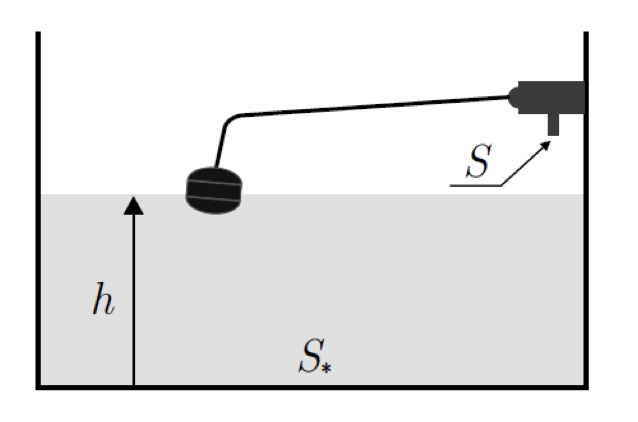
\includegraphics[width = 0.9 \textwidth]{ToileteTank.png}
\end{minipage}
\begin{ans}
$h = h_{\max}(1-e^{-S_0vt/S^*h_{\max}})$
\end{ans}
\end{ex}

\begin{ex}
В цилиндрическом баке с площадью основания $S$ находится вода, уровень которой расположен на высоте $h_0$. Вблизи дна бака имеется небольшое отверстие площадью $s$. Как изменяется со временем уровень воды баке при истечении из отверстия?
\begin{ans}
$h(t) = \left(\sqrt{h_0} - s t \sqrt{g/2} /S \right)^2$
\end{ans}
\end{ex}

\begin{ex}
Вывести дифференциальное уравнение вытекания жидкости из конического сосуда и определить полное время вытекания $T$. Радиус верхнего основания конического сосуда равен $R$, а радиус нижнего основания (отверстия) $a$. Начальная уровень жидкости составляет $H$.
\begin{sol}
Изменение уровня жидкости на высоте \(z\) описывается дифференциальным уравнением
\[S\left( z \right)\frac{{dz}}{{dt}} = q\left( z \right),\]
где \(S\left( z \right)\) -- площадь поперечного сечения сосуда на высоте \(z,\) а \(q\left( z \right)\) -- поток жидкости, зависящий от высоты $z$.

Принимая во внимание геометрию сосуда, можно предположить, что \[q\left( z \right) =  - \pi {a^2}\sqrt {2gz} ,\] где \(a\) -- радиус отверстия на дне конического сосуда. Учитывая, что отверстие достаточно малое, осевое сечение можно рассматривать как треугольник. Из подобия треугольников следует, что \[\frac{R}{H} = \frac{r}{z}.\] Следовательно, площадь поверхности жидкости на высоте \(z\) будет равна
\[
{S\left( z \right) = \pi {r^2} }
= {\pi {\left( {\frac{{Rz}}{H}} \right)^2} }
= {\frac{{\pi {R^2}{z^2}}}{{{H^2}}}.}
\]
Подставляя \(S\left( z \right)\) и \(q\left( z \right)\) в дифференциальное уравнение, имеем:
\[\frac{{\pi {R^2}{z^2}}}{{{H^2}}}\frac{{dz}}{{dt}} =  - \pi {a^2}\sqrt {2gz} .\]
После простых преобразований получаем следующее дифференциальное уравнение:
\[{z^{\large\frac{3}{2}\normalsize}}dz =  - \frac{{{a^2}{H^2}}}{{{R^2}}}\sqrt {2g} dt.\]
Проинтегрируем обе части, учитывая, что уровень жидкости уменьшается от начального значения \(H\) до нуля за время \(T:\)
\[
{\int\limits_H^0 {{z^{\large\frac{3}{2}\normalsize}}dz}  =  - \int\limits_0^T {\frac{{{a^2}{H^2}}}{{{R^2}}}\sqrt {2g} dt} ,}\;\; 
{\Rightarrow \left. {\left( {\frac{{{z^{\large\frac{5}{2}\normalsize}}}}{{\frac{5}{2}}}} \right)} \right|_0^H = \frac{{{a^2}{H^2}}}{{{R^2}}}\sqrt {2g} \left[ {\left. {\left( t \right)} \right|_0^T} \right],}\;\; 
{\Rightarrow \frac{2}{5}{H^{\large\frac{5}{2}\normalsize}} = \frac{{{a^2}{H^2}}}{{{R^2}}}\sqrt {2g} T,}\;\; 
{\Rightarrow \frac{1}{5}\sqrt {\frac{{2H}}{g}}  = \frac{{{a^2}}}{{{R^2}}}T,}\;\; 
{\Rightarrow T = \frac{{{R^2}}}{{5{a^2}}}\sqrt {\frac{{2H}}{g}} .}
\]
\end{sol}
\begin{ans}
$z^{\frac{3}{2}}zt = - \frac{a^2H^2}{R^2}\sqrt{2g}dt$, $T = \frac{R^2}{5a^2}\sqrt{\frac{2H}{g}}$
\end{ans}
\end{ex}

%Юмашев
\begin{ex}
\hspace{0pt} \\
\begin{minipage}{.65\textwidth}
По длинному хорошо растяжимому жгуту, один конец которого прикреплен к стене, а другой оттягивается с постоянной скоростью $u$, ползет муравей. Скорость муравья относительно жгута постоянна и равна $v$ и направлена в сторону движущегося конца жгута. Доберется ли муравей до конца жгута? За какое время? Начальная длина жгута $L_0$, муравей стартует от неподвижного конца.
\end{minipage}
\begin{minipage}{.35\textwidth}
\centering
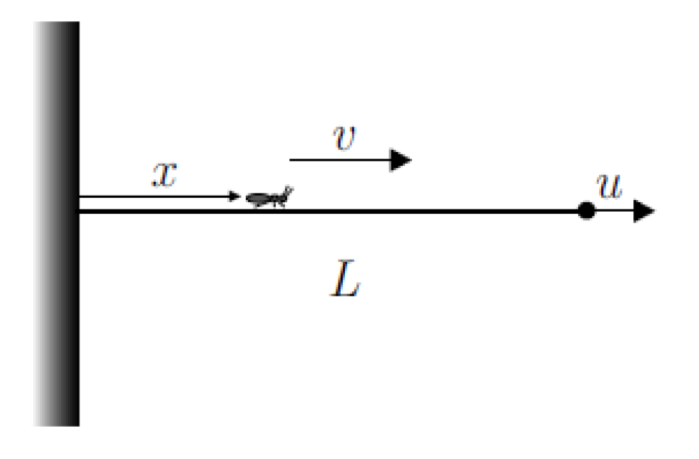
\includegraphics[width = 0.9 \textwidth]{AntAndTow.png}
\end{minipage}
\begin{sol}
см. Юмашев Интегралы и производные в физике
\end{sol}
\begin{ans}
$\tau = L_0(e^{u/v} - 1)/u$
\end{ans}
\end{ex}

%Иродов1.105
\begin{ex}
\hspace{0pt} \\
\begin{minipage}{.65\textwidth}
Небольшую шайбу $A$ положили на наклонную плоскость, составляющую угол $\alpha$ с горизонтом и сообщили начальную скорость $v_0$. Найти зависимость скорости шайбы от угла $\varphi$, если коэффициент трения $k = \tan \alpha$ и в начальный момент $\varphi_0 = \pi/2$.
\end{minipage}
\begin{minipage}{.35\textwidth}
\centering
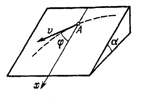
\includegraphics[width = 0.9 \textwidth]{WasherOnSurface.png}
\end{minipage}
\begin{ans}
$v=v_0/(1+\cos \varphi)$
\end{ans}
\end{ex}

%Черепанов
\begin{ex}
Наклонная плоскость имеет угол $\alpha$ с горизонтом. Тело, лежащее на наклонной плоскости, толкнули в горизонтальном направлении с начальной скоростью $v_0$. Коэффициент трения тела о плоскость равен $\mu = k \tan \alpha (k > 1)$. Через какое время тело остановится и какой путь пройдет до остановки?
\begin{ans}
$\tau = \frac{kv_0}{g\sin\alpha(k^2-1)}$, $s = \frac{2v_0^2k^2}{4kg\sin\alpha(k^2-1)}$
\end{ans}
\end{ex}

%Туймадаа
\begin{ex}
С вертикальной скалы высотой $H$ брошен горизонтально со скоростью $v_0$ камень массой $m$. Спустя некоторое время он стал двигаться с постоянной скоростью. Считая, что сила сопротивления воздуха пропорциональна скорости, найти расстояние по горизонтали $L$, на которое камень удалится от скалы в момент падения, и время движения $t$.
\begin{ans}
$L = mv_0/k$, $\tau = kH/mg + m/k$
\end{ans}
\end{ex}

%Черепанов
\begin{ex}
(2007) Бусинка находится в наинизшей точке вертикально расположенной неподвижной шероховатой окружности радиуса $R$. Какую минимальную скорость надо сообщить бусинке, чтобы она достигла горизонтального диаметра окружности? Коэффициент трения равен $\mu$.
\begin{ans}
$v_0^2 = \frac{2gR}{4\mu^2+1}\left( 3\mu e^{\mu \pi} - 2\mu^2 +1\right)$
\end{ans}
\end{ex}

%Черепанов
\begin{ex}
(2008) Сферическая капля воды движется в однородном поле тяжести в среде, в которой за счет конденсации происходит увеличение массы капли, пропорциональное ее поверхности с коэффициентом пропорциональности $\alpha$. Найти скорость капли в зависимости от времени, если в начальный момент времени капля была неподвижна, ее масса равнялась $m_0$. Плотность воды $\rho$.
\begin{ans}
$v=gt/4+g\gamma t (\beta^2t^2+3\beta t \gamma+3\gamma^2)/4(\beta t + \gamma)$, $\beta = 4\pi \alpha(3m/4\pi\rho)^{2/3}/3$, $\gamma = m_0^{1/3}$
\end{ans}
\end{ex}

%Жухарев
\begin{ex} (2008) В данной плоскости движутся две точки: точка 1 движется по прямой с постоянной скоростью $v_1$, а точка 2 – с постоянной по модулю скоростью $v_2$, направленной все время на точку 1. Найти траекторию точки 2 и координату места встречи 1 и 2. Считать, что в начальный момент времени расстояние между точками $y_0$ и $\vec{v_2} \bot \vec{v_1}$.
\begin{ans}
$x=\frac{h}{2(1+u/v)}(\frac{y}{h})^{1+u/v} - \frac{h}{2(1-u/v)}(\frac{y}{h})^{1-u/v} - \frac{h}{2(1+u/v)}+\frac{h}{2(1-u/v)}$, $x_0=h\frac{u}{v}\left(1-\frac{u^2}{v^2}\right)^{-1}$
\end{ans}
\end{ex}

\section{Дополнительные задачи}
\begin{itemize}
\item http://www.math24.ru/прогиб-балки.html Прогиб балки
\item Дифуравнения в механике (Иродов, МФТИ, Morin)
\item Вращательное движение (моменты инерции, сохранение момента импульса)
\item Электростатика (сферы, потенциалы, конденсаторы, задачи Черепанова)
\item ЭМ индукция, сила Ампера (перемычка, замкнута на C, L, R и их комбинации)
\item Переменный ток (Козел)
\end{itemize}